\section{开普勒的行星运动三定律}\label{sec:04.01}
% 123.jpg
牛顿第二定律\lbr 式\eqref{eqn:03.02.01}\rbr 是物体运动的动力学基本规律。然
而,如果没有关于力的详细知识,这个规律是不能应用的。在这
个意义上,我们可以说牛顿第二定律的含义是:研究物体的动力
学的关键是研究物体之间的相互作用力。牛顿在《原理》一书中
曾写道:“我奉献这一作品,作为哲学的数学原理,因为哲学的
全部责任似乎在于——从运动的现象去研究自然界中的力,然后
从这些力去说明现象。”

牛顿使用“从运动的现象去研究力,从力去说明现象”的方
法建立了万有引力定律。

在牛顿之前,人类研究得最多也最清楚的运动现象就是行星
的运行。肉眼可以看到五颗行星:水、金、火、木、土。对这五
颗行星的运动有过长期的观察,特别是丹麦天文学家第谷连续进
行了二十年的仔细观测,他的学生开普勒则花费了大约二十年的
时间分析这些数据。开普勒前后总结出三条行星运动的规律:

(1)所有行星都沿着椭圆轨道运行,太阳则位于这些椭圆的
一个焦点上。这称为轨道定律。

(2)任何行星到太阳的连线在相同的时间内扫过相同的面
积。这称为面积定律
% 124.jpg

(3)任何行星绕太阳运动的周期的平方与该行星的椭圆轨道
的半长轴的立方成正比,即
\begin{equation}\label{eqn:04.01.01}
  T \propto r ^ { 3 / 2 }
\end{equation}
式中,$ T $是行星运动的周期;$ r $是椭圆轨道的半长轴。这称为周期
定律。

表\ref{tab:04.01}~中给出了九个大行星的有关数据。其中是以AU为
单位的,AU是地球轨道的半长轴,称为天文单位,其值是
\begin{equation*}
  1 \symrm{AU} = \num{149.6e8} \text{ 公里}
\end{equation*}

图\ref{fig:04.01}~画出了$ \ln T $与$ \ln r $之间的关系。它是一条直线,斜率为
3/2,就是式\eqref{eqn:04.01.01}~的图示。
\begin{figure}[h]
  \centering
  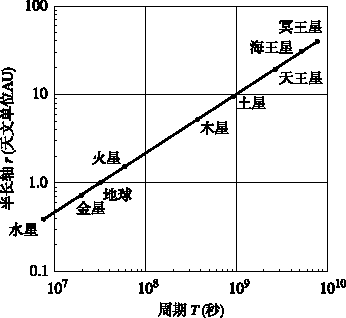
\includegraphics{figure/fig04.01}
  \caption{行星的$T\mbox{-}r$周期}
  \label{fig:04.01}
  \vspace{-0.5em}
\end{figure}

根据行星运动的这三条规律,牛顿得出了万有引力。在讲万
有引力之前,我们要说明,“从运动现象去研究力”这种方法并
不是唯一的。

\begin{table}[h]
  \caption{行星的周期和轨道半长轴的值}
  \label{tab:04.01}
  \zihao{-5}
  \begin{tblr}{row{2-Z}={rowsep=1pt},colsep=2.5em,colspec={c|ZZ}}
    \toprule
    行\quad 星 & $r\text{(AU)}$ & $T\text{(日)}$ \\
    \midrule
    水\quad 星 & 0.387099       & 87.969         \\
    金\quad 星 & 0.723332       & 224.701        \\
    地\quad 球 & 1.000000       & 365.256        \\
    火\quad 星 & 1.523691       & 686.980        \\
    木\quad 星 & 5.202803       & 4332.589       \\
    土\quad 星 & 9.53884        & 10759.22       \\
    天王星     & 19.1819        & 30685.4        \\
    海王星     & 30.0578        & 60189          \\
    冥王星     & 39.44          & 90465          \\
    \bottomrule
  \end{tblr}
\vspace{-1em}
\end{table}
开普勒本人在得到上述的行星运动的规律之后,也曾企图寻
找运动的原因,来解释行星运动的现象。但是他并不着眼于力,
而是着眼于对称性。开普勒首先要解释行星半长轴为什么有表
\ref{tab:04.01}所列出的值。他认为这是宇宙的对称和和谐的表现。他设计了
% 125.jpg
一个由正多面体构成的宇宙。如图\ref{fig:04.02}所示,土星的轨道在最外的
一个大圆上;在该球内作一内接的正六面体,木星轨道在该六面体
的内切球面上在这球内再作一正四面体,火星轨道则在该四面体
的内切球面上;相继地,再在这球面内作一内接正十二面体,地球
轨道在这十二面体的内切球面上;再继续作一内接的正%
\begin{figure}[h]
  \centering
  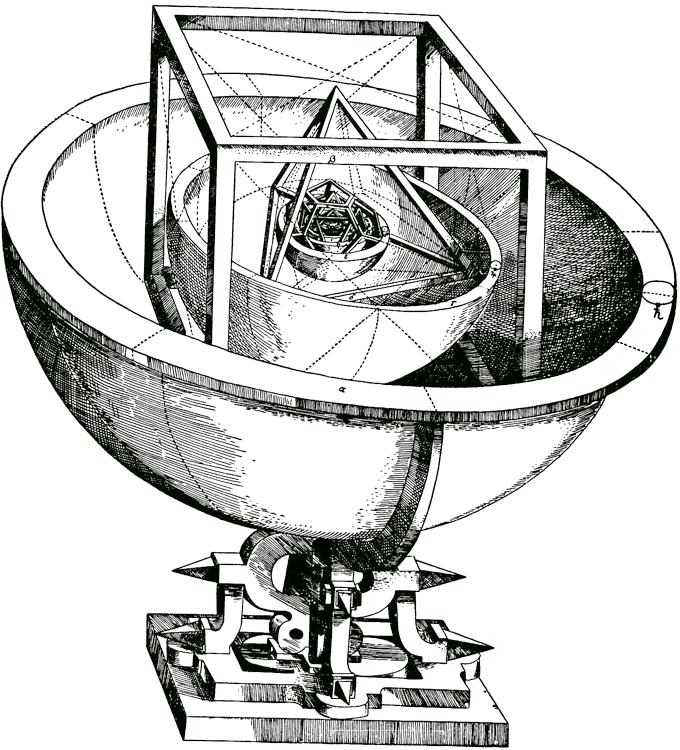
\includegraphics[height=14.5em]{figure/fig04.02a}
\end{figure}%
\begin{figure}[h]
  \centering
  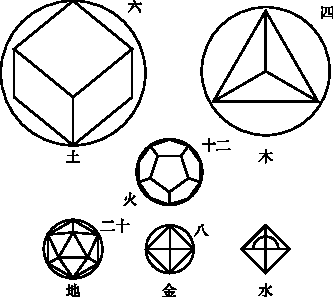
\includegraphics{figure/fig04.02b}
  \caption{开普勒的宇宙模型}
  \label{fig:04.02}
\end{figure}%
二十面体,金星轨道就在二十面体的内切球面上;最后,作内接的正八面体,
其内切球面就是水星的轨道所在之处。

我们知道,正多面体的种类是不多的,用上述的一系列正多
面体的套装,开普勒能给出符合观测的行星轨道半径之间的比例,
不能不说这是一个很有意义的尝试。虽然现在已经证明,开普勒
的解释并不正确,但是这个事例告诉我们,“从运动的现象去研
究对称性”,也是一种有价值的方法。的确,在一些现代物理的
研究中往往是首先着眼于对称性的。

